\newpage

\section{迁移学习前沿}

从我们上述介绍的多种迁移学习方法来看,领域自适应(Domain Adaptation)作为迁移学习的重要分类,在近年来已经取得了大量的研究成果。但是,迁移学习仍然是一个活跃的领域,仍然有大量的问题没有被很好地解决。

本节我们简要介绍一些迁移学习领域较新的研究成果。并且,管中窥豹,展望迁移学习未来可能的研究方向。

\subsection{机器智能与人类经验结合迁移}

机器学习的目的是让机器从众多的数据中发掘知识,从而可以指导人的行为。这样看来,似乎“全自动”是我们的终极目标。我们理想中的机器学习系统,似乎就应该完全不依赖于人的干预,靠算法和数据就能完成所有的任务。Google Deepmind公司最新发布的AlphaZero~\cite{silver2017mastering}就实现了这样的愿景:\textit{算法完全不依赖于人提供知识,从零开始掌握围棋知识,最终打败人类围棋冠军。}随着机器学习的发展,似乎人的角色也会越来越不重要。

然而,在目前看来,机器想完全不依赖于人的经验,就必须付出巨大的时间和计算代价。普通人也许根本无法掌握这样的能力。那么,如果在机器智能中,特别是迁移学习的机器智能中,加入人的经验,可以大幅度提高算法的训练水平,这岂不是我们喜闻乐见的?

来自斯坦福大学的研究人员2017年发表在人工智能顶级会议AAAI上的研究成果就率先实践了这一想法~\cite{stewart2017label}。研究人员提出了一种无需人工标注的神经网络,对视频数据进行分析预测。在该成果中,研究人员的目标是用神经网络预测扔出的枕头的下落轨迹。不同于传统的神经网络需要大量标注,该方法完全不使用人工标注。取而代之的是,将人类的知识赋予神经网络。

我们都知道,抛出的物体往往会沿着\textit{抛物线}的轨迹进行运动。这就是研究人员所利用的核心知识。计算机对于这一点并不知情。因此,在网络中,如果加入抛物线这一基本的先验知识,则会极大地促进网络的训练。并且,最终会取得比单纯依赖算法本身更好的效果。

我们认为将机器智能与人类经验结合起来的迁移学习应该是未来的发展方向之一。期待这方面有更多的研究成果发表。

\subsection{传递式迁移学习}

迁移学习的核心是找到两个领域的相似性。这是成功进行迁移的保证。但是,假如我们的领域数据本身就不存在相似性,或者相似性极小,这时候就很容易出现负迁移。负迁移是迁移学习研究中极力需要避免的。

我们由两个领域的相似性推广开来,其实世间万事万物都有一定的联系。表面上看似无关的两个领域,它们也可以由中间的领域构成联系。也就是一种传递式的相似性。例如,领域A和领域B从表面上看,完全不相似。那么,是否可以找到中间的一个领域C,领域C与A和B都有一定的相似性?这样,知识原来不能直接从领域A迁移到领域B,加入C以后,就可以先从A迁移到C,再从C迁移到B。这就是传递迁移学习。

香港科技大学杨强教授的团队率先在2015年数据挖掘顶级会议KDD上提出了这一概念:Transitive transfer learning~\cite{tan2015transitive}。随后,作者又进行了进一步的扩展,将三个领域的迁移,扩展到多个领域。这也是符合我们认知的:原先完全不相似的两个领域,如果它们中间存在若干领域都与这两个领域相似,那么就可以构成一条相似性链条,知识就可以进行链式的迁移。作者提出了远领域的迁移学习(Distant Domain Transfer Learning)~\cite{tan2017distant},用卷积神经网络解决了这一问题。

在远领域迁移学习中,作者做出了看起来并不符合常人认知的实验:由人脸图片训练好的分类器,迁移识别飞机图像。研究人员采用了人脸和飞机中间的一系列类别,例如头像、头盔、水壶、交通工具等。在实验中,算法自动地选择相似的领域进行迁移。结果表明,在初始迁移阶段,算法选择的大多是与源领域较为相似的类别;随着迁移的进行,算法会越来越倾向于选择与目标领域相似的类别。这也是符合我们的基本认知的。最终的对比实验表明,这种远领域的迁移学习比直接训练分类器的精度会有极大的提升。图~\ref{fig-future-ddtl}展示了知识迁移的过程。

\begin{figure}[htbp]
	\centering
	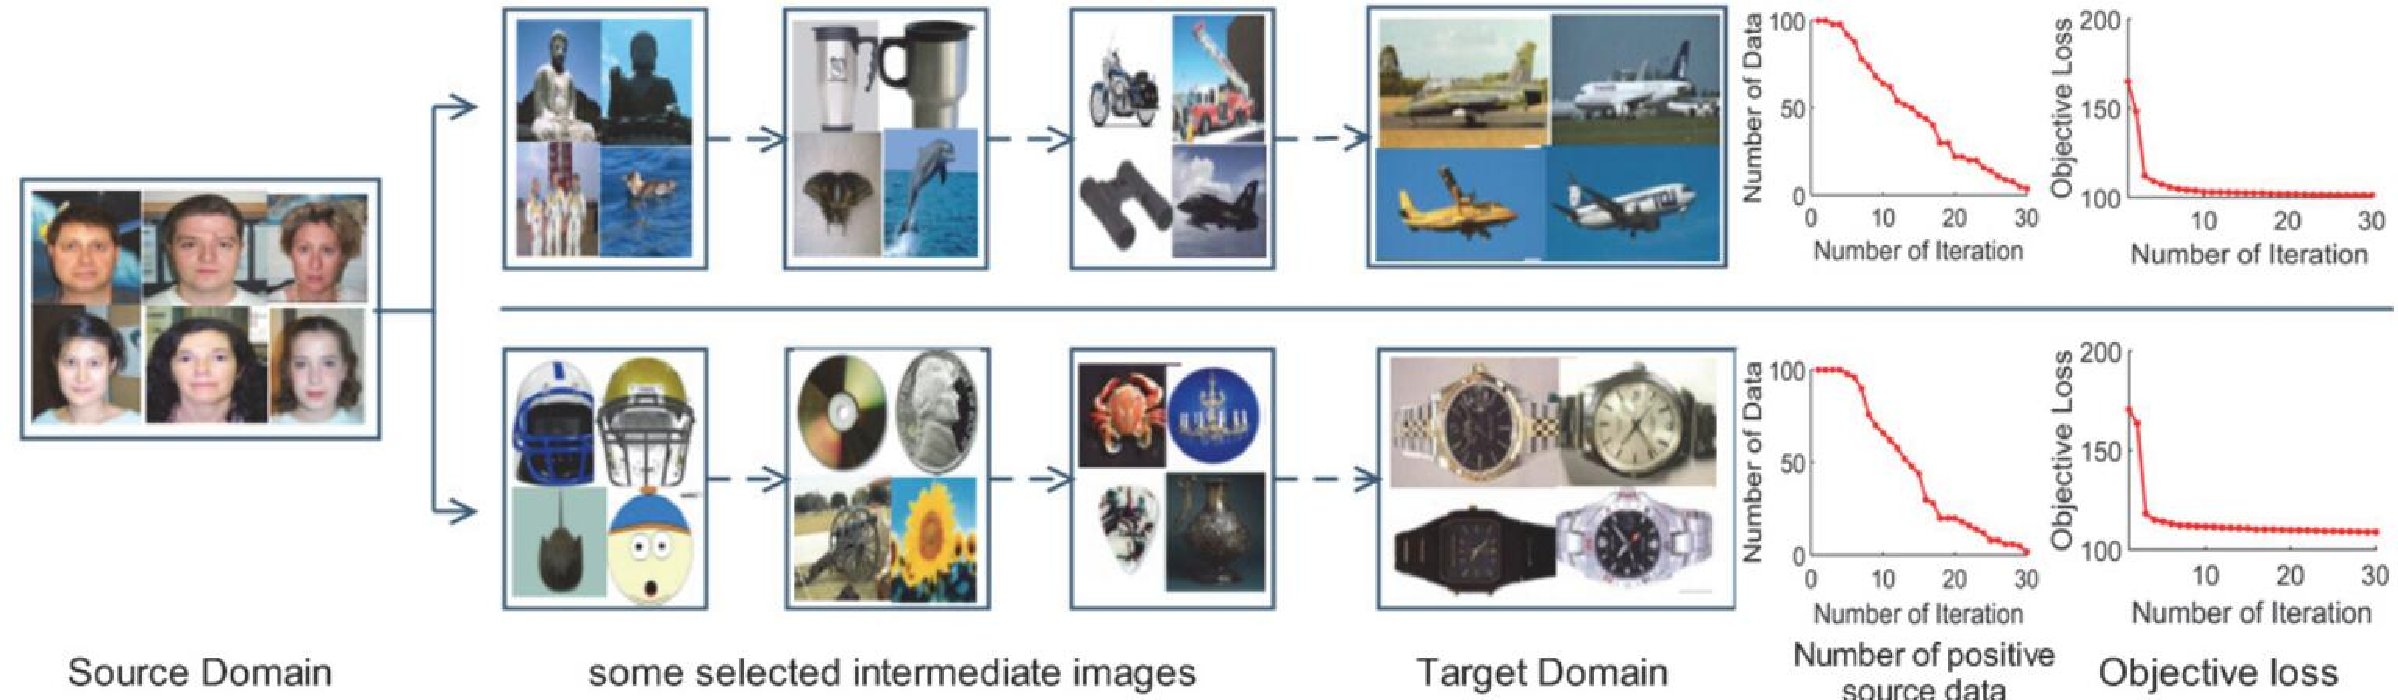
\includegraphics[scale=0.35]{./figures/fig-future-ddtl.pdf}
	\caption{远领域迁移学习示意图}
	\label{fig-future-ddtl}
\end{figure}

传递迁移学习目前的研究成果还十分稀少。我们期待这一领域会有更多好的成果出现。

\subsection{终身迁移学习}

我们在进行迁移学习时,往往不知道应该选择怎么样的算法。通常都通过人为地不断尝试来确定要用的方法。这个过程无疑是浪费时间,而且充满了不确定性。已有的迁移学习方法,基本都是这样。我们在拿到一个新问题时,如何选择迁移学习算法达到最好的效果?从人的学习过程中来说,人总是可以从以前的经验中学习知识。那么,既然我们已经实验了很多次迁移学习算法,我们能不能让机器也可以从我们这些实验中选择知识?这是符合我们人类认知的:不可能每遇到一个新问题,我们就从头开始做吧?

同样是来自香港科技大学杨强教授团队就开始了这一方面的研究工作。他们提出一种学习迁移(L2T, Learning to Transfer)的框架~\cite{wei2017learning},解决\textit{何时迁移、要迁移什么、怎么迁移}的问题。方法分为两个部分:从已有的迁移学习方法和结果中学习迁移的经验,然后再把这些学习到的经验应用到新来的数据。

首先要明确学习目标。跟以前的迁移学习方法都有所不同,以往的方法都是要学习最好的迁移函数,而这个问题的目标是要使得方法尽可能地具有泛化能力。因此,它的学习目标是:\textbf{以往的经验}!对的,就是经验。这也是符合我们人类认知的。我们一般都是知道的越多,这个人越厉害(当然,《权利的游戏》里的Jon Snow除外,因为他什么也不知道)。因此,这个方法的目标就是要尽可能多地从以往的迁移知识中学习经验,使之对于后来的问题具有最好的泛化能力。 

那么\textit{什么是迁移的经验}?这个在文中叫做transfer learning experience。作者这样定义:$Ee=(S_e,T_e,a_e,l_e)$。其中,$S_e,T_e$分别是源域和目标域,这个我们都知道。$a_e$表示一个迁移学习算法,这个算法有个下标叫$e$,表示它是第$e$种算法。与之对应,选择了这种算法,它对不迁移情况下的表现有个提升效果,这个效果就叫做$le$。

总结一下,什么叫迁移学习的经验?就是说,在一对迁移任务中,我选择了哪种算法后,这种算法对于我任务效果有多少提升。这个东西,就叫做迁移!这和我们人类学习也是具有相似性的:人们常说,失败是成功之母,爱因斯坦说,我实验了2000多种材料做灯泡都是失败的,但是我最起码知道了这2000多种材料不适合做灯泡!这就是人类的经验!我们人类就是从跌倒中爬起,从失败中总结教训,然后不断进步。学习算法也可以! 

后面的过程就是,综合性地学习这个迁移过程,使得算法根据以往的经验,得到一个特征变换矩阵$\mathbf{W}$。学习到了这个变换矩阵以后,下一步的工作就是要把学习到的东西应用于新来的数据。如何针对新来的数据进行迁移?我们本能地要利用刚刚学习到的这个$\mathbf{W}$。但是不要忘了,这个变换矩阵只是对旧的那些经验学习到的,对新的数据可能效果不好,不能直接用。怎么办?我们要更新它!

这里要注意的是,针对新来的数据,我们的这个变换矩阵应该是有所改变的:这也对,数据变了,当然变换矩阵就要变。那么,如何更新?作者在这里提出的方法是,新的矩阵应该是能在新的数据上表现效果最好的那个。这时,我们的问题就完成了。 

图~\ref{fig-future-l2t}简要表示了该算法的学习过程。

\begin{figure}[htbp]
	\centering
	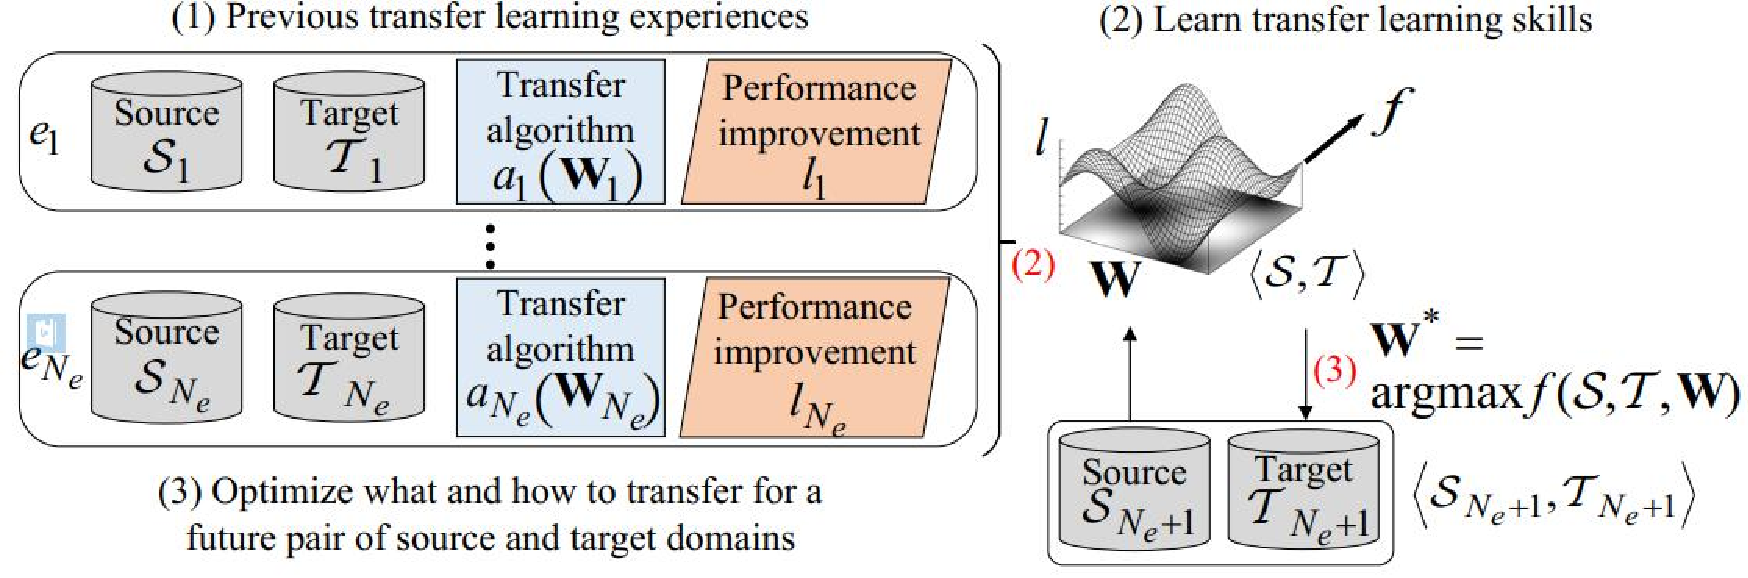
\includegraphics[scale=0.35]{./figures/fig-future-l2t.pdf}
	\caption{终身迁移学习示意图}
	\label{fig-future-l2t}
\end{figure}

这有点类似增量学习的工作:模型针对新数据不断更新优化。这部分的研究才刚刚开始。

\subsection{在线迁移学习}

我们都知道迁移学习可以用来解决训练数据缺失的问题,很多迁移学习方法都获得了长足的进步。给定一个要学习的目标域数据,我们可以用已知标签的源域数据来给这个目标域数据构造一个分类器。但是这些方法都存在很大的一个问题:它们都是采用离线方式(offline)进行的。什么是离线方式?就是说,一开始,源域和目标域数据都是给出来的,我们直接做完迁移,这个过程就结束了。We are done。

但是真实的应用往往不是这样的:数据往往是一点一点源源不断送来的。也就是说,我们一开始的时候,也许只有源域数据,目标域数据要一点一点才能过来。这就是所谓的“在线迁移学习”。这个概念脱胎于“在线学习”的模式,在线学习是机器学习中一个重要的研究概念。

就目前来说,在线迁移学习方面的工作较少。第一篇在线迁移学习的工作由新加坡管理大学的Steven Hoi发表在2010年的机器学习顶级会议ICML上。作者提出了OTL框架~\cite{zhao2010otl},可以对同构和异构数据很好地进行迁移学习。

近年来,研究者发表了一些在线迁移学习相关的文章。其中包括在多个源域和目标域上的OTL~\cite{wu2017online,yan2017online},在线特征选择迁移变换~\cite{wang2014online,zhang2017online},在线样本集成迁移~\cite{gao2012online,patilknowledge}等。

特别地,\cite{jaini2016online}提出了用贝叶斯的方法学习在线的HMM迁移学习模型,并应用于行为识别、睡眠监测,以及未来流量分析。这是一篇有代表性的应用工作。

总结来看,目前在在线迁移学习方面的研究工作总体较少,发展空间巨大。在可以预见的未来,我们期待更多的研究者可以从事这一领域的研究。将深度网络、对抗学习结合入在线迁移学习,使得这一领域的发展越来越好。

\subsection{迁移强化学习}

Google公司的AlphaGo系列在围棋方面的成就让\textit{强化学习}这一术语变得炙手可热。用深度神经网络来进行强化学习也理所当然地成为了研究热点之一。不同于传统的机器学习需要大量的标签才可以训练学习模型,强化学习采用的是\textit{边获得样例边学习}的方式。特定的反馈函数决定了算法的最优决策。

深度强化学习同时也面临着重大的挑战:没有足够的训练数据。在这个方面,迁移学习却可以利用其他数据上训练好的模型帮助训练。尽管迁移学习已经被应用于强化学习~\cite{taylor2009transfer},但是它的发展空间仍然还很大。强化学习在自动驾驶、机器人、路径规划等领域正发挥着越来越重要的作用。我们期待在未来有更多的研究成果可以问世。

\subsection{迁移学习的可解释性}

深度学习取得众多突破性成果的同时,其面临的可解释性不强却始终是一个挑战。现有的深度学习方法还停留在"黑盒子"阶段,无法产生足够有说服力的解释。同样的,迁移学习也有这个问题。即使世间万物都有联系,它们更深层次的关系也尚未得到探索。领域之间的相似性也正如同海森堡"测不准原理"一般无法给出有效的结论。为什么领域A和领域B更相似,而和领域C较不相似?目前也只是停留在经验阶段,缺乏有效的理论证明。

另外,迁移学习算法也存在着可解释性弱的问题。现有的算法均只是完成了一个迁移学习任务。但是在学习过程中,知识是如何进行迁移的,这一点还有待进一步的实验和理论验证。最近,澳大利亚悉尼大学的研究者们发表在国际人工智能联合会IJCAI 2017上的研究成果有助于理解特征是如何迁移的~\cite{liu2017understanding}。

用深度网络来做迁移学习,其可解释性同样有待探索。最近,Google Brain的研究者们提出了神经网络的"核磁共振"现象~\footnote{\url{https://github.com/tensorflow/lucid}},对神经网络的可解释性进行了有趣的探索。

